\section{Results and Analysis} \label{sec:results}
% 1. Accuracy (F1 + MCC) auf SICK und eSNLI einzeln nach Kategorien
% 2. Auf Bias überprüfen: Vergleich vom Modell für wichtig erachtete Token mit von Menschen als wichitg erachtete Tokens
% Visualisierungen:
% - Confusion Matrix (Gentrennt nach Phänomenen)
% - Tabellen Interpretability Metriken (siehe ferret)
In this section the results of our experiments are described and thoroughly analyzed. The results are grouped according to the hypotheses they support.

\subsection{Testing H1}
To test the knowledge contained in \acp{PLM}, we devise prompts that allow for \ac{NLI} predictions, as described in \autoref{sec:meth:probing}. The results obtained using the prompting methods are shown in \autoref{tab:res:prompting}. The word group chosen a priori from the list of discourse markers performs best in F$_1$-Score and second best in \ac{MCC}. The simple word group performs worst in \ac{MCC} but second best in F$_1$-Score. The tuned word group performs best in \ac{MCC} and slightly worse than the simple word group in F$_1$-Score. The difference in F$_1$-Score between a priori and the other word groups is far bigger than the gaps in the \ac{MCC} scores. As the discrepancy is great, we added a metric, the balanced accuracy, to the evaluation that should also be better for imbalanced data than the F$_1$-Score and sometimes more informative than the \ac{MCC} \cite{mccBad}. The balanced accuracy is calculated as the macro-average of the true positive rate of each class \cite{bacc}. Looking at the results in the additional metric, they confirm the ranking obtained by using the \ac{MCC} values. Using this additional fact, we conclude that the \ac{MCC} values are more trustworthy than the F$_1$-Scores for this task.
\begin{table}[ht!]
    \centering
    \caption{Prediction performance when using prompting with different word groups on the \acs{SICK} dataset. The best result is shown in \textbf{bold} and the second-best is \underline{underlined}.}
    \begin{tabular}{l c c c}
        \toprule
        \multicolumn{1}{c}{Word Group} & \acs{MCC} & $\text{F}_1$ & BAcc\\
        \midrule
        A Priori & $\underline{25.51}\%$ & $\mathbf{54.31\%}$ & $\underline{54.11}\%$ \\
        Simple & $20.56\%$ & $\underline{34.40\%}$ & $45.67\%$ \\
        Tuned & $\mathbf{29.11\%}$ & $34.08\%$ & $\mathbf{55.73\%}$\\
        \bottomrule
    \end{tabular}
    \label{tab:res:prompting}
\end{table}

Looking at the resulting \ac{MCC} scores, we can see the expected ordering: The a priori chosen word group is better than the simple words that do not fit into the sentence and the tuned words perform best, as they are tuned on \ac{MultiNLI} to perform better. Interestingly, all approaches, even the simple approach, perform much better than random, which would be an \ac{MCC} of $0$. Nonetheless, compared to the \ac{MCC} score of the fine-tuned model, which is $49.49\%$, the results of using prompting are far worse, even when specifically tuning the prompt words.

\subsection{Testing H2}
Figure~\ref{fig:ferret-sample} shows the explanations for the finetuned model's classification of a sample from the validation split of the \ac{e-SNLI} dataset obtained using ferret \cite{ferret}. It can be seen that the meaning of the quantifiers in this sample is not considered by the model: The usage of quantifiers in this sample makes it a contradiction but the model attaches high importance only to the quantifier \enquote{all} whereas \enquote{several} has very low importance to the model. The existence of such samples where the model only poorly captures the importance of quantifiers shows that the model is biased after fine-tuning on \ac{MultiNLI}.

\begin{figure*}[h!]
    \centering
    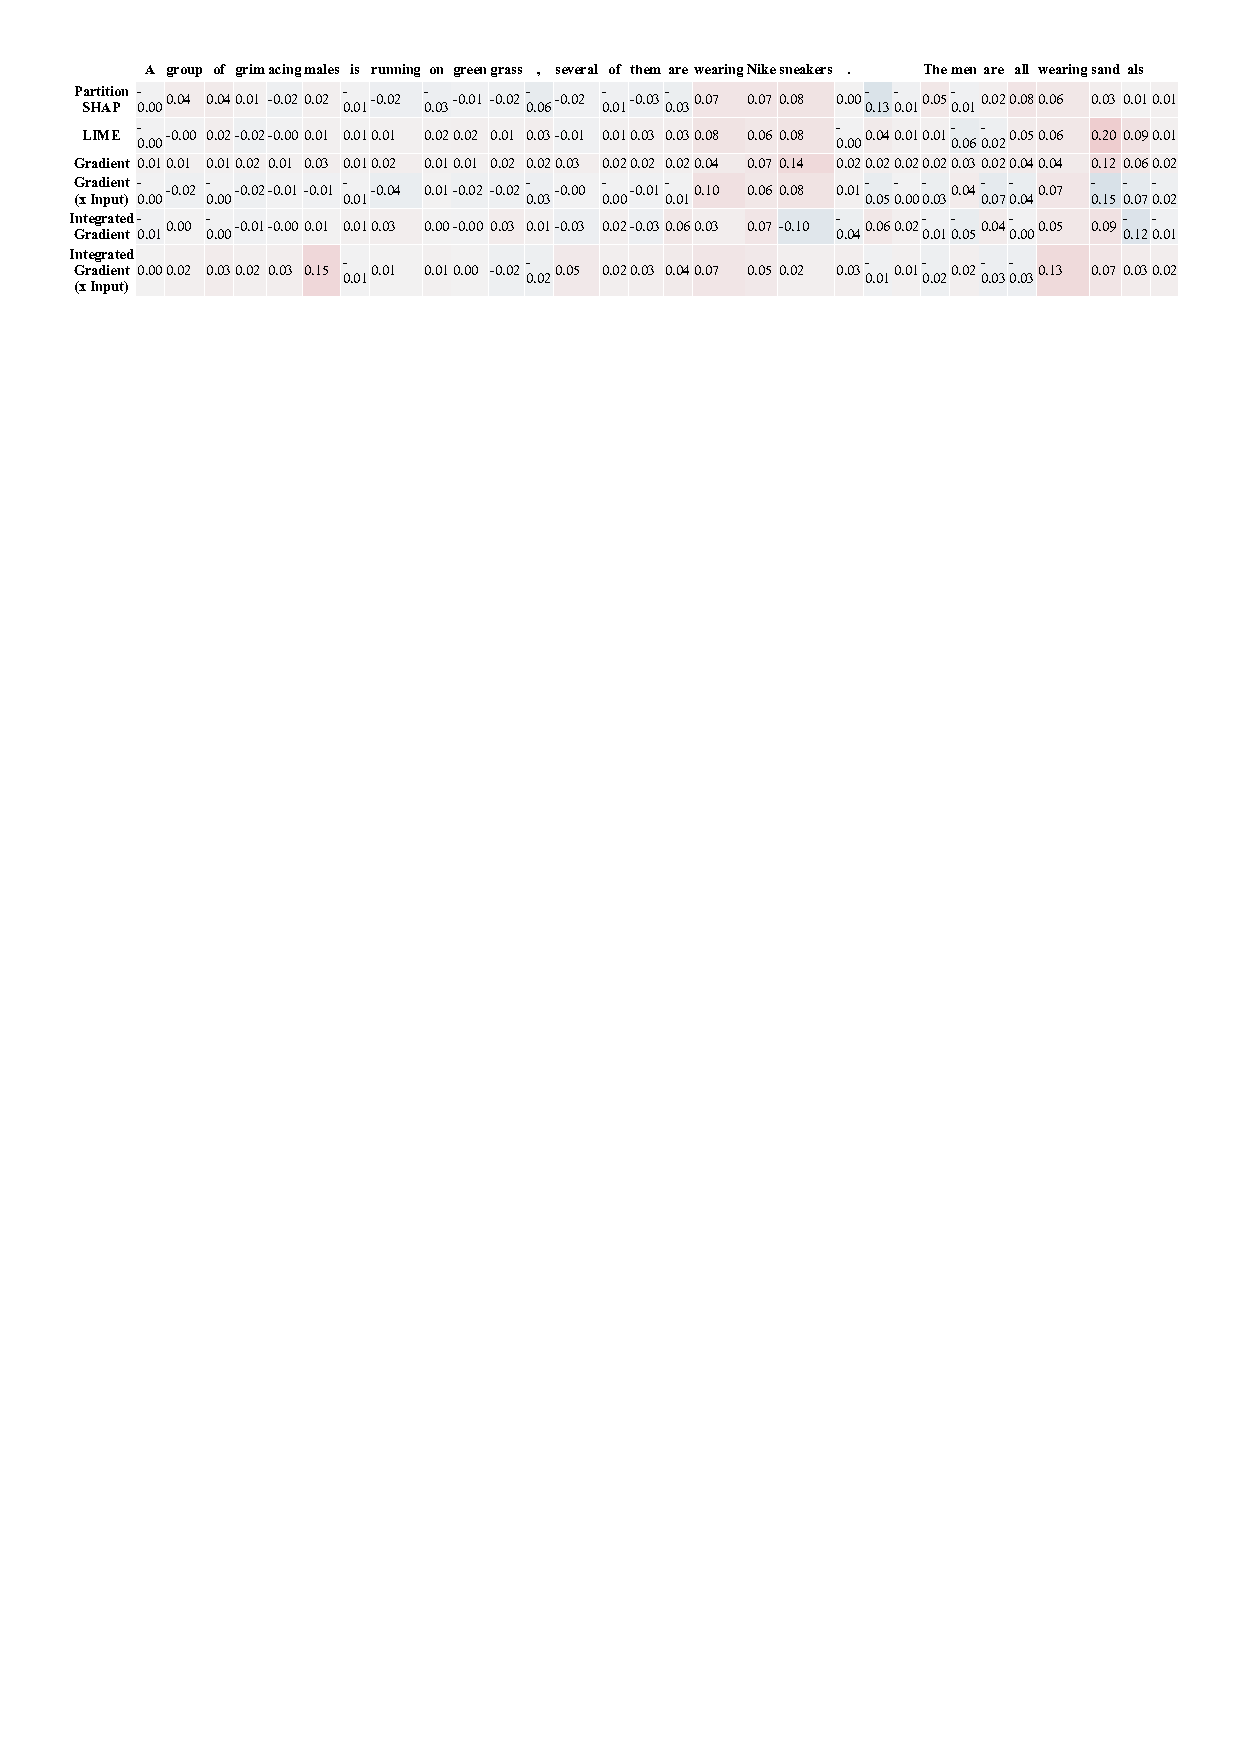
\includegraphics[width=\textwidth]{./images/ferret_sample.pdf}
    \caption{Expamle of a bad explanation}
    \label{fig:ferret-sample}
\end{figure*}

\subsection{Testing H3}
Figure~\ref{fig:metric-heatmap-phenomena-mcc} depicts the \ac{MCC} scores separated by linguistic phenomena for our model trained on different datasets as described in \autoref{sub:experiments-h4} to show the different predictive performance of the models. The results for the hypothesis-only model were measured on the validation-matched split of \ac{MultiNLI}.

\begin{figure}[h!]
    \centering
    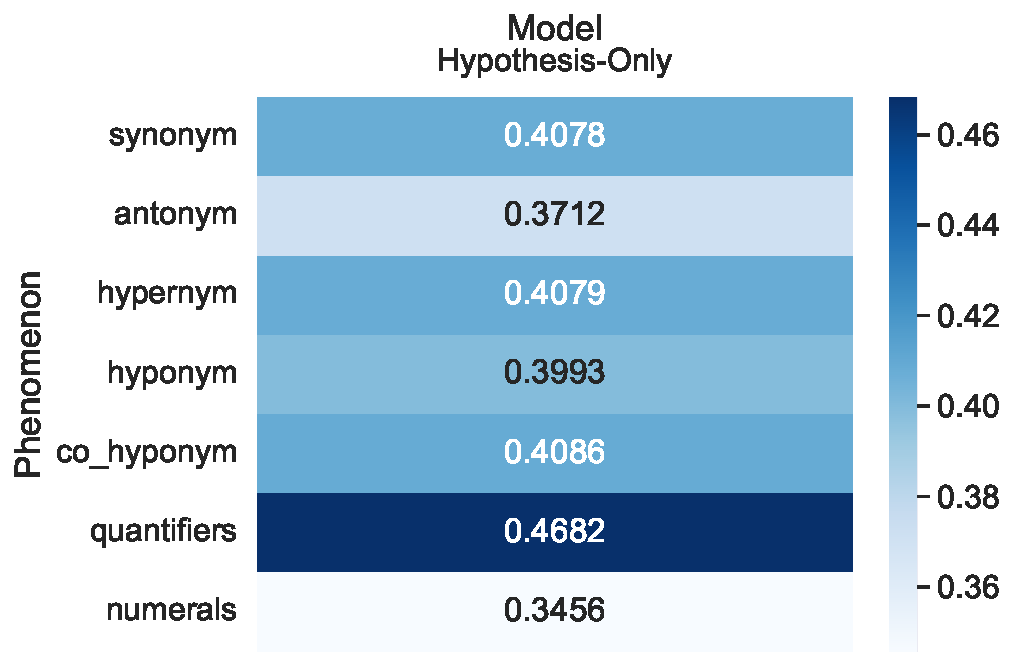
\includegraphics[width=0.9\columnwidth]{./images/metric_heatmaps_phenomena/important_words/hypothesis_only_matthews_correlation.pdf}
    \caption{Matthews Correlation Coefficients for the model trained on different datasets separated by linguistic phenomena}
    \label{fig:metric-heatmap-phenomena-mcc}
\end{figure}

In general, the hypothesis-only model shows the expected poor performance: For the phenomena of synonym, hypernym, hyponym and co-hyponym the \ac{MCC} is around $0.4$. The exceptions are antonym, quantifiers and numerals. The model performs particularly poorly on samples that contain antonyms and even worse for numerals. This behavior can be explained by the distribution of phenomena in the dataset shown in \autoref{tab:mnli:phenomena}: Antonyms are found in only $18874$ samples in the training split of \ac{MultiNLI} and numerals only in the hypotheses of $38168$ samples. This makes them the two rarest phenomena in the dataset. 

\begin{table}[ht]
    \centering
    \caption{Phenomena distribution of the hypothesis of the training split of \ac{MultiNLI}}
    \small
    \begin{tabular}{l r}
        \toprule
        \multicolumn{1}{c}{Phenomenon} &  \multicolumn{1}{c}{Number of Samples} \\
        \midrule
        Synonym & $339763$ \\
        Antonym & $18874$ \\
        Hypernym & $117645$ \\
        Hyponym & $124984$ \\
        Co-Hyponym & $381690$ \\
        Quantifier & $48526$ \\
        Numeral & $38168$ \\
        \bottomrule
    \end{tabular}
    \label{tab:mnli:phenomena}
\end{table}

Also comparably rare are samples which contain quantifiers. Nevertheless, the model performs best on samples with an \ac{MCC} of about $0.46$. Since the model cannot possibly determine the meaning of the quantifier for the classification without knowledge of the premise this result is a clear indicator of a bias in the samples that contain quantifiers.

\subsection{Testing H4}
\begin{table}[ht!]
    \centering
    \caption{Prediction performance of our fine-tuned models on the \acs{SICK} dataset. The best result is shown in \textbf{bold} and the second-best is \underline{underlined}.}
    \begin{tabular}{l c c}
        \toprule
        \multicolumn{1}{c}{Model} & \acs{MCC} & $\text{F}_1$ \\
        \midrule
        Base & $49.49\%$ & $56.60\%$ \\
        Hypothesis-Only\tablefootnote{Average of three runs with different seeds} & $14.13\%$ & $40.02\%$ \\
        Filtered $2/3$ & $46.21\%$ & $54.12\%$ \\
        Filtered $2/3$ longer & $36.17\%$ & $52.85\%$ \\
        Filtered $3/3$ & $48.73\%$ & $56.94\%$ \\
        Filtered $3/3$ longer & $\mathbf{52.31\%}$ & $\mathbf{62.04\%}$ \\
        Ensembled & $\underline{51.65\%}$ & $\underline{59.88\%}$ \\
        Recast & n/a & n/a \\
        \bottomrule
    \end{tabular}
\end{table}

Figure~\ref{fig:metric-heatmap-phenomena-mcc} depicts the \ac{MCC} scores separated by linguistic phenomena for our model trained on different datasets as described in \autoref{sub:experiments-h4} to show the different predictive performance of the models.

\begin{figure}[ht]
    \centering
    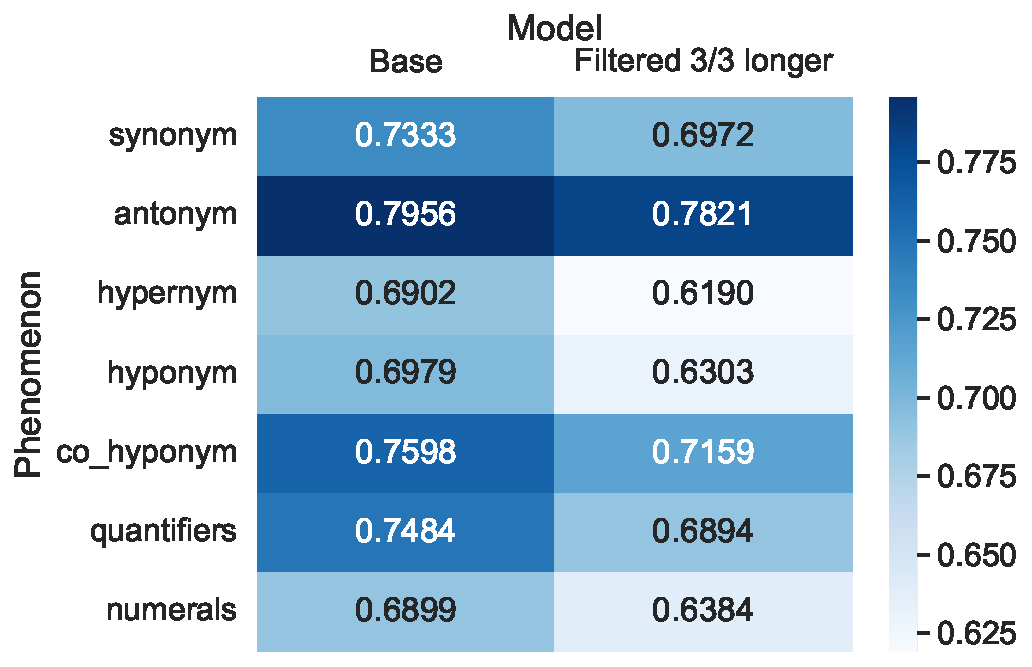
\includegraphics[width=0.9\columnwidth]{./images/metric_heatmaps_phenomena/important_words/base_filtered_matthews_correlation.pdf}
    \caption{Matthews Correlation Coefficients for the model trained on different datasets separated by linguistic phenomena}
    \label{fig:metric-heatmap-phenomena-mcc}
\end{figure}

The Hypothesis-Only model shows the expected poor performance but performs comparably well on samples that contain antonyms which indicates a bias in these samples as the model cannot detect the presence of an antonym for the right reasons without knowing the premise. The improved performance of the Filtered 3/3 longer model shows that this bias can be mitigated by the naive approach of removing the biased samples.

\subsection{Testing H5}
